\documentclass[a4paper, 11pt]{exam}
\usepackage[T1]{fontenc}
\usepackage{titling}
\usepackage{url}
\usepackage{amsmath,amsthm,amssymb}
\usepackage{graphicx}
\usepackage{graphics}
\usepackage{listings}
\usepackage{color} % Required for custom colors
\usepackage[dvipsnames]{xcolor}
\usepackage{tabularx}
\usepackage{ragged2e}
\usepackage{courier}
\usepackage{textcomp}
\usepackage{circuitikz}
\usepackage{tikz}
\usepackage{enumitem}
\usepackage{karnaugh-map}
\usepackage{bytefield}
\usepackage{mathrsfs}
\usepackage{cancel}
\usepackage[linesnumbered,ruled,vlined]{algorithm2e}
\usepackage{hyperref}
\usepackage{amsmath}
\usepackage{my_styles}  % This includes my custom style definitions for code

\newcommand{\invlaplace}[1]{%
\mathscr{L}^{-1}\left\{#1\right\}
}
\newcommand{\laplace}[1]{%
\mathscr{L}\left\{#1\right\}
}
\newcommand{\fourier}[1]{%
\mathscr{F}\left\{#1\right\}
}

\newcommand{\ztransform}[1]{%
\mathscr{Z}\left\{#1\right\}
}

\newcommand{\subtitle}[1]{%
  \posttitle{%
    \par\end{center}
    \begin{center}\large#1\end{center}
    }%
}

\usepackage{environ}

\NewEnviron{eqnsection}[2]{%
  \newcommand{\myvspace}{#1}%
  \vspace{\myvspace}%
  \begin{align*}
  \intertext{#2}
  \BODY
  \end{align*}%
  \vspace{\myvspace}%
}



\newlist{myenumerate}{enumerate}{2}
\setlist[myenumerate,1]{label=\roman*)}
\setlist[myenumerate,2]{label=\alph*)}



\newcommand\tab[1][1cm]{\hspace*{#1}}

\renewcommand{\labelenumi}{\alph{enumi})}

\title{Team Project: Octave Band Filtering}
\subtitle{ECE 6530: Digital Signal Processing \\
\today\\}
\author{ Tyler Bytendorp \and Miguel Gomez \and Chase Griswold \and Benjamin Hayes \and\\
University of Utah Electrical and Computer Engineering}
\date{Due Date: Dec 5, 2023}

\begin{document}
\maketitle
\noindent

\section*{5.1 Octave Bands}
This bit was taken care of in Matlab and this is the function to set up the filter bands table. The results are below and a copy of the code is included in appendix A:
\begin{table}[!ht]
\centering
\begin{tabular}{|l|c|c|c|c|c|c|c|c|}
\hline
val [units] & $O_1$  & $O_2$ & $O_3$ & $O_4$ & $O_5$ & $O_6$ & $O_7$ & $O_8$ \\
\hline
Lower (Hz)   & 32.703 & 65.406   & 130.81   & 261.63   & 523.25   & 1046.5   & 2093     & 4186    \\
\hline
Lower (Rad)  & 0.025685 & 0.05137  & 0.10274  & 0.20548  & 0.41096  & 0.82192  & 1.6438   & 3.2877  \\
\hline
Upper (Hz)   & 61.735 & 123.47   & 246.94   & 493.88   & 987.77   & 1975.5   & 3951.1   & 7902.1  \\
\hline
Upper (Rad) & 0.048487 & 0.096974 & 0.19395  & 0.3879   & 0.77579  & 1.5516   & 3.1032   & 6.2063  \\
\hline
Center (Hz)  & 47.219 & 94.439   & 188.88   & 377.75   & 755.51   & 1511     & 3022     & 6044.1  \\
\hline
Center (Rad) & 0.037086 & 0.074172 & 0.14834  & 0.29669  & 0.59338  & 1.1868   & 2.3735   & 4.747   \\
\hline
\end{tabular}
\caption{Frequency Ranges for Octaves 1 to 8 starting with $O_1$}
\end{table}
Since we have a limit on the bands we can recognize that arises from the use of the sampling freq of $8kHz$, we can only obtain unique detection for the set of Octaves whose frequencies are below the Nyquist rate of $\frac{fs}{2}$ or $4kHz$. Or, $O_7$ in the table above.

\section*{5.2 Octave Filter Bank}
 Comment on the selectivity of the bandpass filters, i.e., use the frequency response (passbands and stopbands) to explain how the filter passes one octave while rejecting the others. Are the filter’s passbands narrow enough so that only one octave lies in the passband and the others are in
 the stop-band?
\\ Comment here and then do the next bit. need a plot from 5.2 that Tyler made. our beta is 1\\
The band pass filter bank was put together in python and has the added benefit of being more portable than the use of Matlab for this application. These are the results from the creation of the x signal needed to pass on to the filter bank. Defining the expression below:
\begin{center}
  \[
    x(t) =
    \begin{cases}
      \ \ \ \ \ \ \ \ \ \ \cos{(2\pi\cdot 220 t)} & 0.0 < t \le 0.25 , \\
      \ \ \ \ \ \ \ \ \ \ \cos{(2\pi\cdot 880 t)} & 0.3 < t \le 0.55 , \\
      \cos{(2\pi\cdot 440 t)} + \cos{(2\pi\cdot 880 t)} & 0.60 < t \le 0.85\\
      \ \ \ \ \ \ \ \ \ \ \ \ \ \ \ \ \ \ \ 0\ \ & \text{otherwise}
    \end{cases}
    \]
\end{center}
\newpage
and now the code to do this along with the plot showing the data is what we expect:\\  
\begin{figure}[h!]
  \centering
  \hspace*{-1.5cm}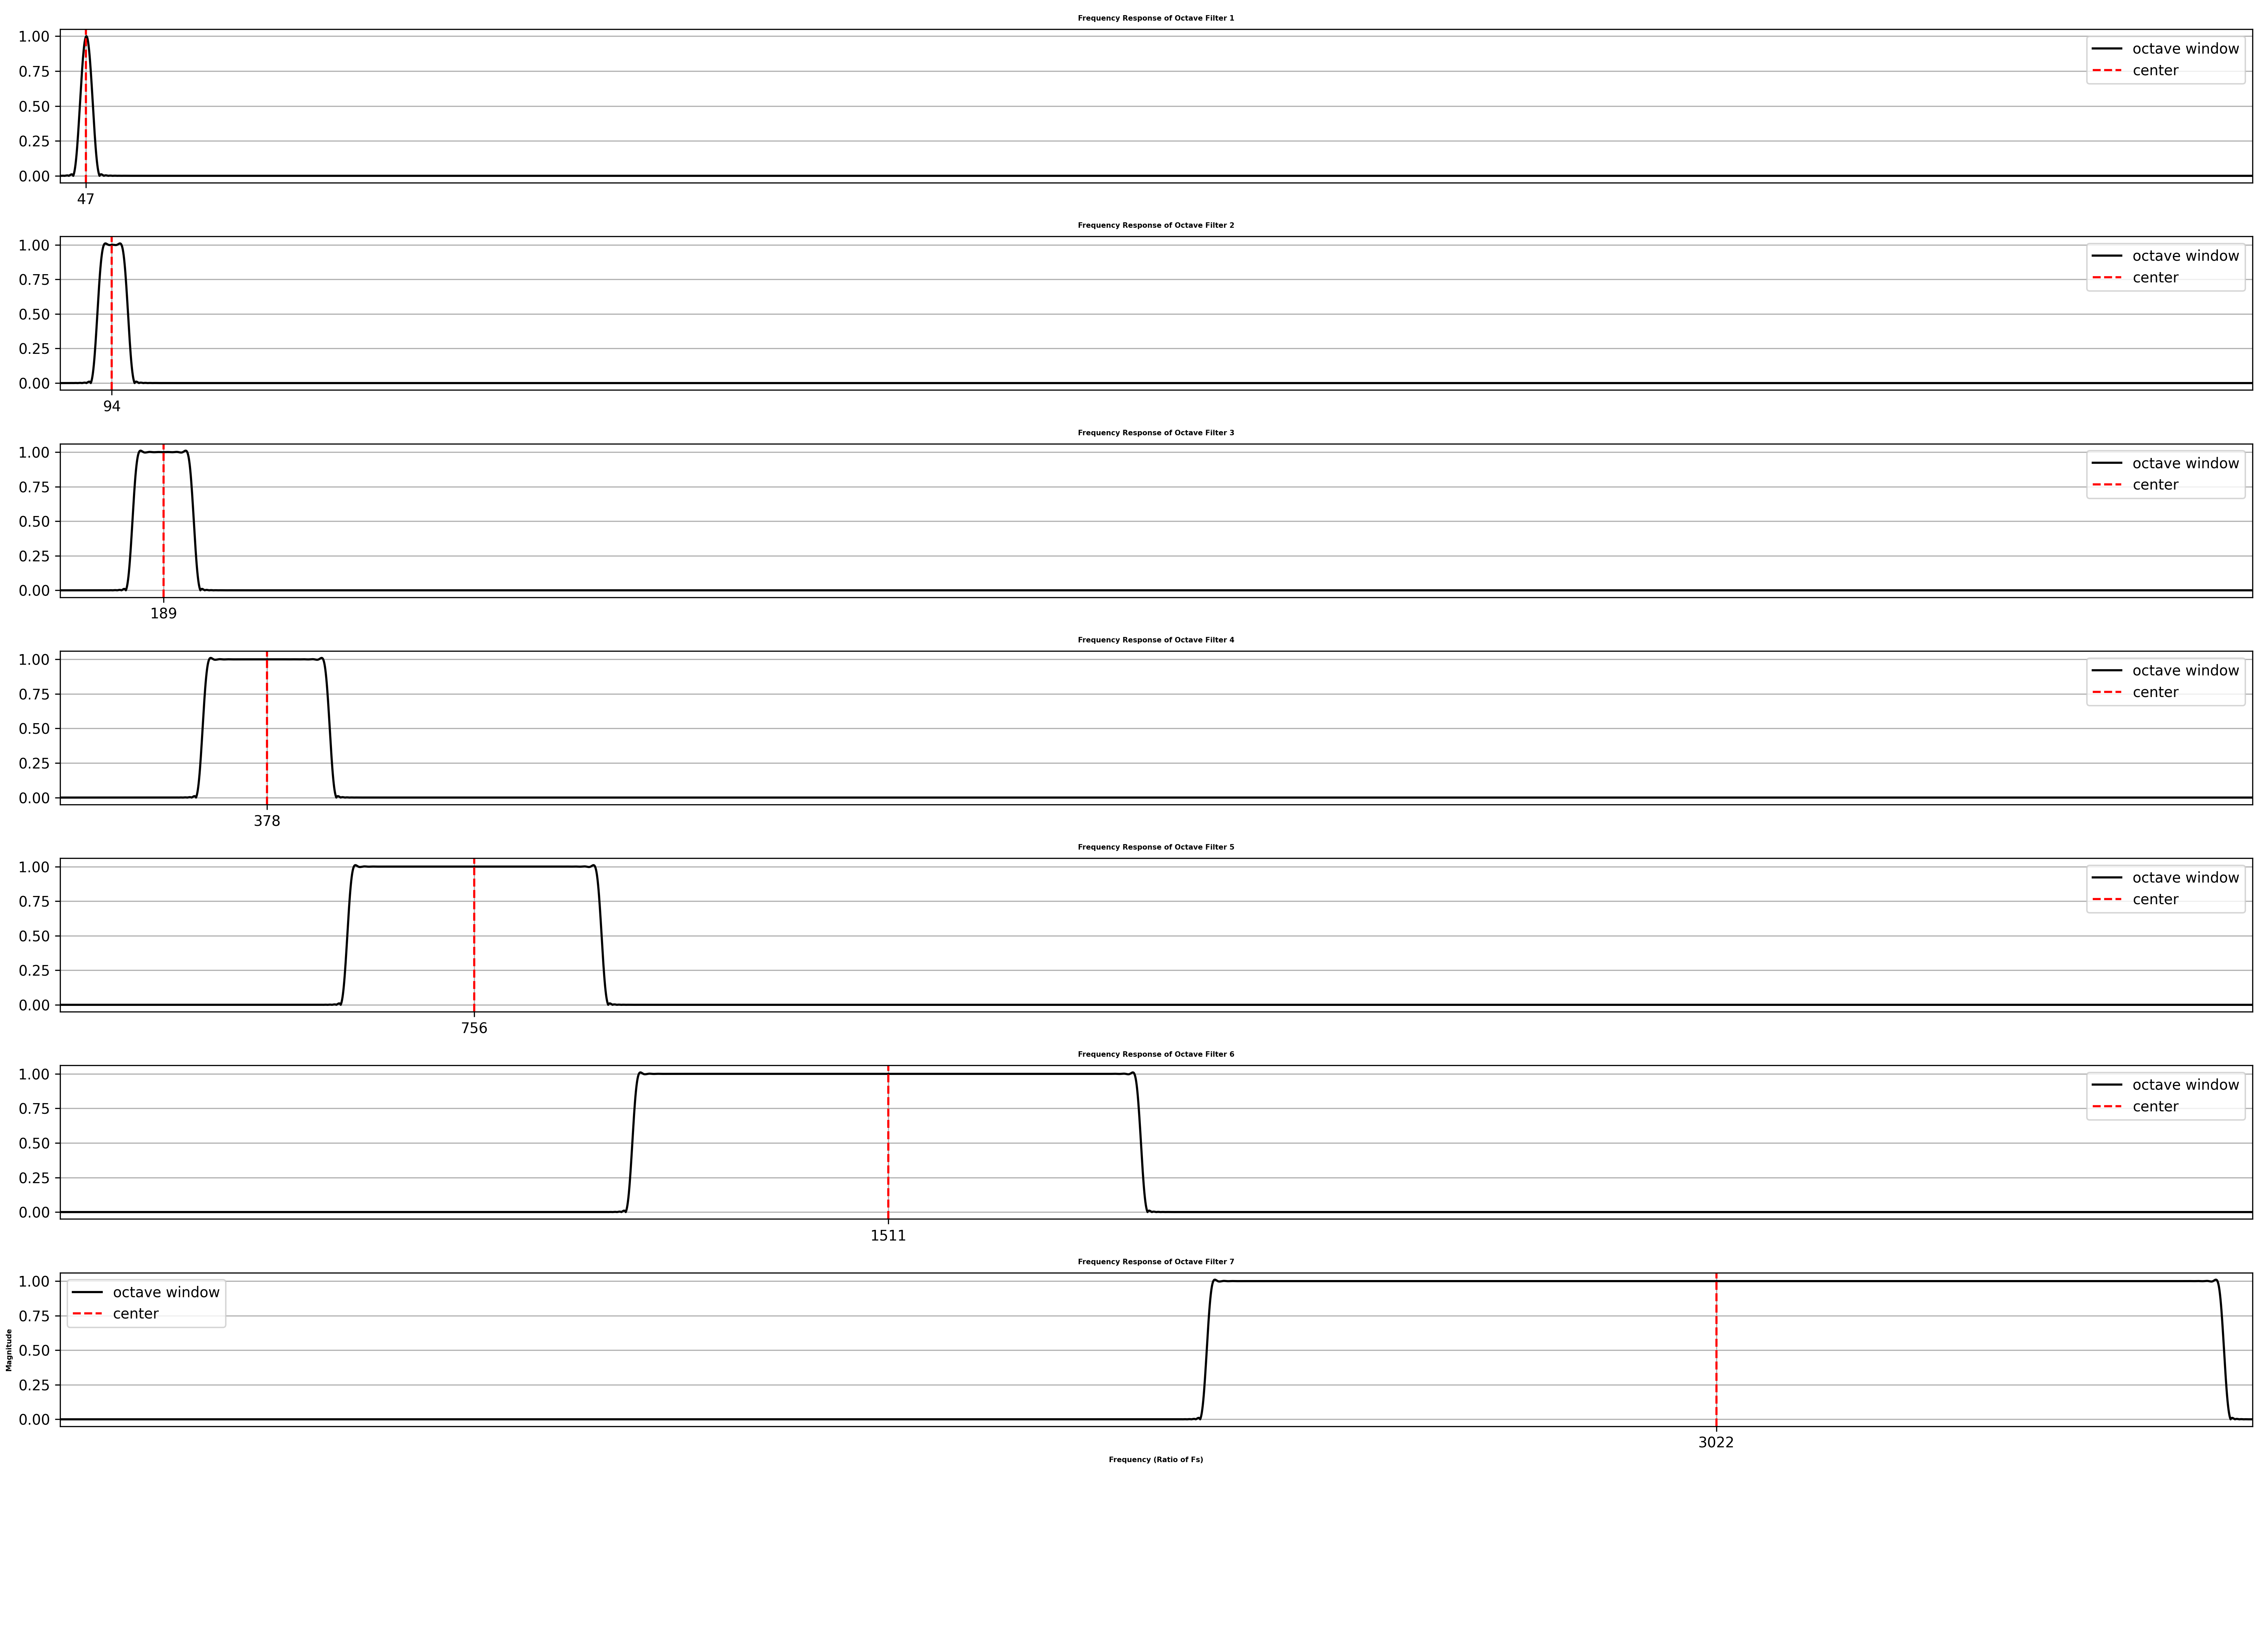
\includegraphics[width=18cm]{../images/freq_data.png}
  \caption{plot for all BPF's}
  \label{fig:bandpass}
\end{figure}
\newline
The filters above in fig. \ref{fig:bandpass} begin at a center of $47Hz$ but we only need to worry about the subsequent ones that we were asked for. Aligned at their centers is a vertical line and a tick mark indicating the center frequency. this bank of filters is what we will use to pass the time data created in the equation above. 
\newpage
\begin{figure}[h!]
  \centering
  \hspace*{-1.5cm}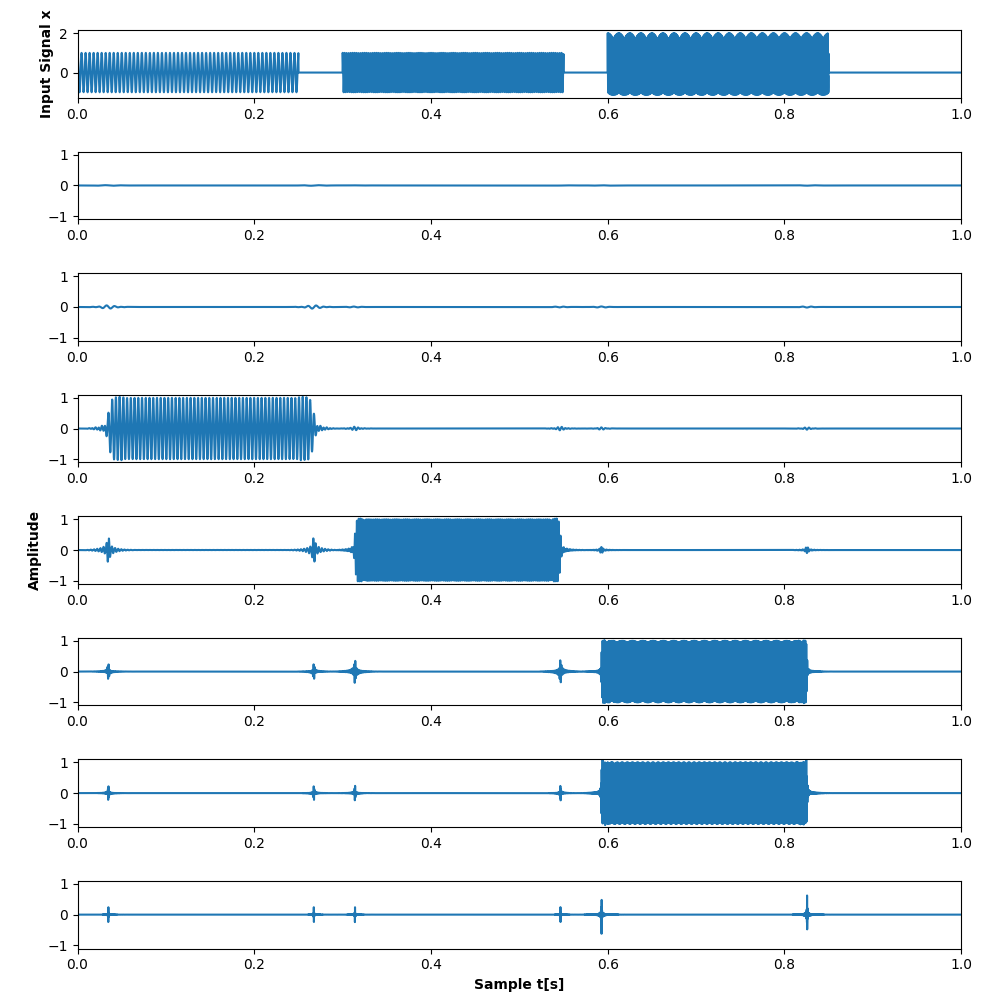
\includegraphics[width=17cm]{../images/time_data.png}
  \caption{plot for all BPF's processing the time data at the top}
  \label{fig:time_data}
\end{figure}
Filters one and two do not pass anything since they are both too low to capture the first freq of $220Hz$, but the third has a center of $189Hz$, meaning it does capture the first frequency. In all cases, we can see that the transition points have the characteristic peaks associated with instant changes in frequency. Any instant change results in a sharp change which corresponds to an infinite number of frequencies. the third filter is capable of capturing the $880Hz$, the fourth captures the $1760Hz$ in superposition with the $880Hz$, and no signal is passed through the last except the transients that appear in all filters.
\newpage
\begin{figure}[h!]
  \centering
  \hspace*{-1.5cm}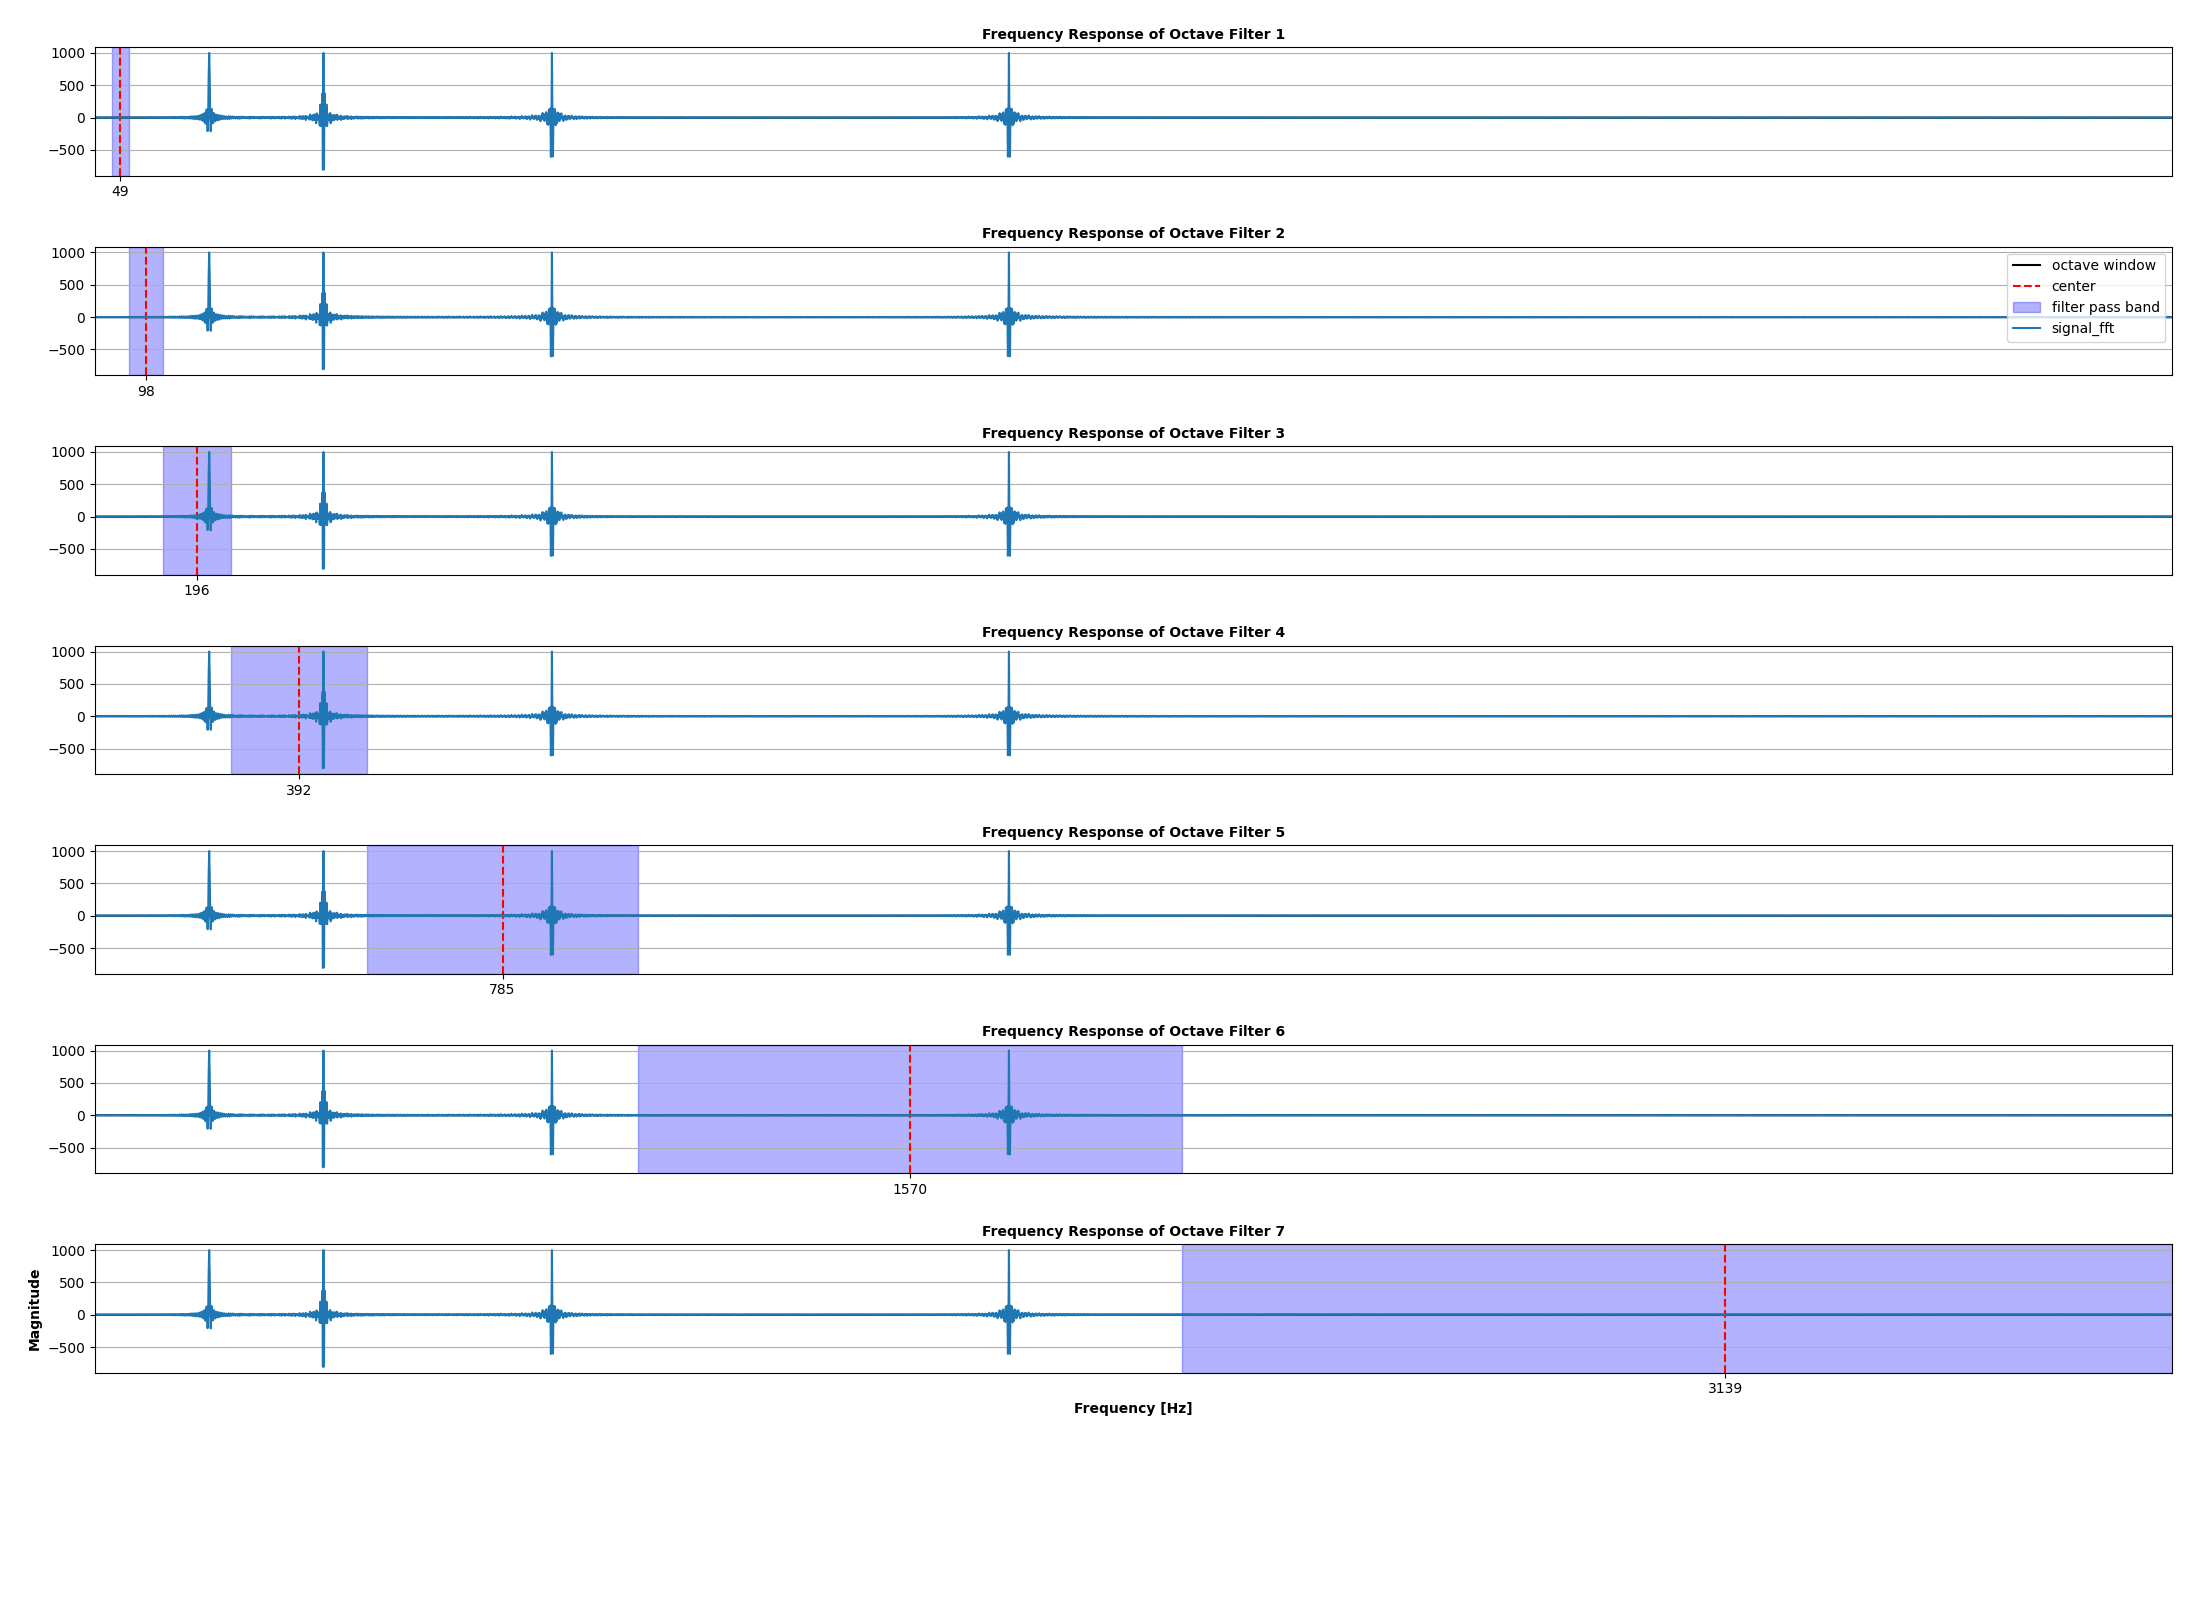
\includegraphics[width=17cm]{../images/fft_freqdata.png}
  \caption{plot for all BPF's bandpass regions}
  \label{fig:bandpass_regions}
\end{figure}
In this figure, it is easier to see that the band-pass filters correctly capture the frequencies that we see in the time plot of fig. \ref{fig:time_data}. In the figure above fig. \ref{fig:bandpass_regions}, we can see that the filters that do not capture any signal do not have an overlapping note peak in the shaded region. However, the ones that we see with a signal passed through them do have a corresponding note in the shaded band-pass region. 

\subsection{Creating the FIR Filters}
To create the FIR filters, we used a python class shown in subsection \ref{app_sub_FIR_create}. The class works by first defining $N$, the number of points to be used in the FIR filter. We then declare the pass band region, the frequencies we wish for the FIR filter to pass through while the others are rejected. This is shown in fig. \ref{define_freqs}. Effectively, we are specifying the desired frequency response of the FIR filter but only using $N$ number of points to define the filter in the frequency domain.

\newpage
\begin{figure}[h!]
  \centering
  \hspace*{-1.5cm}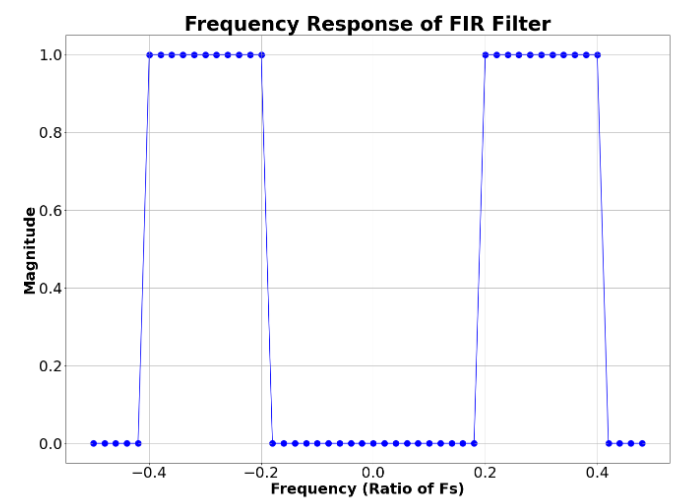
\includegraphics[width=17cm]{../images/define_freqs.png}
  \caption{Band-pass region of the FIR filter being created. The filter response is specified by N number of points where N is the length of the FIR filter being created.}
  \label{fig:define_freqs}
\end{figure}

After defining the frequency response with $N$ number of points, we need to also ensure that the frequency response is symmetric about the y-axis. This ensures that our FIR filter will be purely real. To obtain the time domain FIR filter, we then take the inverse fourier transform of the $N$ number of points specifying the frequency response. The FIR filter corresponding to the frequency response shown in \ref{fig:define_freqs} above.

\newpage
\section*{Appendix A}
\subsection{Matlab Code}
\begin{lstlisting}[language=Matlab]
function print_octaves(n,fs)
% n should be a range relative to A4. ex: -1:1 gives A3,A4,A5
A4 = 440;
C4 = A4.*2.^(-9./12);
B4 = A4.*2.^(2./12);
Octaves = 2.^n;
Cs = C4.*Octaves;
Bs = B4.*Octaves;
n_range = 0:length(n)-1;
Centers = (Cs + Bs)./2;
cell(size(Centers));
octave_array = arrayfun(@(x) sprintf('Octave %d', x), n_range, 'UniformOutput', false);
w_Cs = Cs.*2.*pi./fs;
w_Bs = Bs.*2.*pi./fs;
w_Centers = Centers.*2.*pi./fs;
rows = {'Lower (Hz)','Lower (Rad)','Upper (Hz)','Upper (Rad)','Center (Hz)','Center (Rad)'};
% Summarize data in a table
T = array2table([Cs; w_Cs; Bs; w_Bs; Centers; w_Centers],'VariableNames',octave_array,'RowName',rows);
disp(T)
disp('Hz are not normalized.')
disp('Radians are normalized by sampling frequency.')
end 
\end{lstlisting}
\subsection{Python Code}
\begin{lstlisting}[language=Python]
from util.OctaveBandFilt import OctaveBandFilter, ourOctaveBandFilter
from util.FIR_filter import FIRFilter
import numpy as np
import matplotlib.pyplot as plt
from rich import print
import math

fontsize = 20

def calculate_grid_dimensions(n):
    columns = round(math.sqrt(n))
    rows = math.ceil(n / columns)
    return rows, columns


def calculate_octave_ranges(base_freq, num_octaves, sample_rate):
    octave_ranges = []
    for i in range(num_octaves+1):
        fmin = base_freq * (2 ** i)  # Minimum frequency for the octave
        fmax = base_freq * (2 ** ((i*12+11)/12))  # Maximum frequency for the octave

        # Normalize the frequencies
        fmin_normalized = fmin
        fmax_normalized = fmax

        octave_ranges.append((fmin_normalized, fmax_normalized))
    return octave_ranges


def windowed_sinc(filter_length, low_freq, high_freq):
    n = np.arange(filter_length)
    mid = (filter_length - 1) / 2
    window = np.hamming(filter_length)

    # Debugging: Print frequency values
    print("low_freq:", low_freq)
    print("high_freq:", high_freq)

    sinc_low = np.sinc(2 * low_freq * (n - mid))
    sinc_high = np.sinc(2 * high_freq * (n - mid))
    bp_filter = sinc_high - sinc_low

    # Debugging: Print sinc function outputs
    print("sinc_low sample values:", sinc_low[:5])
    print("sinc_high sample values:", sinc_high[:5])

    bp_filter *= window
    bp_filter_sum = np.sum(bp_filter)

    # Debugging: Check for zero sum
    print("bp_filter sum after window:", bp_filter_sum)
    if bp_filter_sum == 0:
        bp_filter_sum = 1  # To avoid division by zero

    bp_filter /= bp_filter_sum

    # Debugging: Final check
    print("Final bp_filter sample values:", bp_filter[:5])
    return bp_filter


# Example usage
filter_length = 150  # A typical length for FIR filters
center_frequency = 220  # Center frequency in Hz
sampling_frequency = 12000  # Sampling frequency in Hz

# Recreating the OctaveBandFilter instance with the updated class definition
octave_filter = OctaveBandFilter(filter_length, center_frequency, sampling_frequency)
octave_filter.calculate_coefficients()


# Recreating the OctaveBandFilter instance with the updated class definition
ourOctave_filter = ourOctaveBandFilter(filter_length, center_frequency, sampling_frequency, windowed_sinc)
ourOctave_filter.calculate_coefficients()
print("Coefficients:", ourOctave_filter.coefficients)
# Generating a test signal - a simple sine wave at the center frequency
test_signal = np.sin(2 * np.pi * center_frequency / sampling_frequency * np.arange(0, sampling_frequency))

# Applying the filter to the test signal
filtered_signal = octave_filter.apply_filter(test_signal)
# Applying the filter to the test signal
ourFiltered_signal = ourOctave_filter.apply_filter(test_signal)


def generate_fm_signal(sampling_frequency, duration, start_freq, end_freq):
    """
    Generate a frequency modulated (FM) signal.
    """
    t = np.arange(0, duration, 1/sampling_frequency)  # Time vector
    instantaneous_frequency = np.linspace(start_freq, end_freq, len(t))
    phase = 2 * np.pi * np.cumsum(instantaneous_frequency) / sampling_frequency
    signal = np.sin(phase)
    return signal


# Parameters for the OctaveBandFilter
filter_length = 150
center_frequency = 440  # Center frequency in Hz
sampling_frequency = 8000  # Sampling frequency in Hz
# Lambda function for windowed sinc



# Creating the filter instance and calculating coefficients
Octave_filter = OctaveBandFilter(filter_length, center_frequency, sampling_frequency)
Octave_filter.calculate_coefficients()
# Creating the filter instance and calculating coefficients
ourOctave_filter = ourOctaveBandFilter(filter_length, center_frequency, sampling_frequency, windowed_sinc)
ourOctave_filter.calculate_coefficients()

# Generating an FM signal
duration = 5  # 1 second duration
start_freq = 1  # Starting frequency of 0 Hz
end_freq = 4 * ourOctave_filter.center_frequency  # Ending at twice the center frequency of the filter
fm_signal = generate_fm_signal(sampling_frequency, duration, start_freq, end_freq)

# Filtering the FM signal
filtered_fm_signal = Octave_filter.apply_filter(fm_signal)
# Filtering the FM signal
ourFiltered_fm_signal = ourOctave_filter.apply_filter(fm_signal)

# Sample rate and base frequency
base_freq = 32.703*1  # Starting frequency of the first octave
# Calculate octave ranges
num_octaves = 6
octave_ranges = calculate_octave_ranges(base_freq, num_octaves, 8000)


# Create a set of filters
N = 1000
filters = [FIRFilter(N, fmin=fmin, fmax=fmax, padding_factor=9, fs=8000) for fmin, fmax in octave_ranges]
num_filters = len(filters)
#filters = [FIRFilter(N, fmin=fmin*N, fmax=fmax*N, padding_factor=9) for fmin, fmax in octave_ranges]
print(f"octave ranges: {octave_ranges}")
# Calculate grid size
total_subplots = num_filters
rows, cols = calculate_grid_dimensions(total_subplots)
print(f"rows: {rows}")
print(f"cols: {cols}")
# Create a figure for plotting
fig = plt.figure(figsize=(22, 16))

mids = [(b+a)/2 for a, b in octave_ranges]
print(mids)
# Plot each filter's response
for i, filter in enumerate(filters):
    # Calculate position
    position = i * 2 + 1  # Position for frequency response plot
    x = mids[i]
    filter.plot_filter(fig, num_filters+1, 1, i+1)
    plt.axvline(x=x, ymin=0, ymax=1, color='r', linestyle='--')
    plt.legend(['octave window', 'center'])
    plt.xticks([x])
    ax = plt.gca()
    ax.set_xlim([0, filter.fs/2])

plt.tight_layout()
plt.show(block=False)
plt.savefig("freq_data_2.png", dpi=300, transparent=False)
plt.close()
num_octaves = 6
octave_ranges = calculate_octave_ranges(base_freq, num_octaves, 1000)
filters = [FIRFilter(N, fmin=fmin, fmax=fmax, padding_factor=9, fs=8000) for fmin, fmax in octave_ranges]
num_filters = len(filters)
# Generate the signal 5.2
fs = 8000
t1 = np.linspace(0, 0.25, int(fs*0.25), endpoint=False)
t2 = np.linspace(0.3, 0.55, int(fs*0.25), endpoint=False)
t3 = np.linspace(0.6, 0.85, int(fs*0.25), endpoint=False)
t_end = np.linspace(0.85, 1, int(fs*0.15), endpoint=False)

x1 = np.cos(2*np.pi*220*t1)
x2 = np.cos(2*np.pi*440*t2)
x3 = np.cos(2*np.pi*880*t3) + np.cos(2*np.pi*1760*t3)

zero_padding = np.zeros(int(fs*0.05))
zeros_end = np.zeros(int(fs*0.15))
x = np.concatenate((x1, zero_padding, x2, zero_padding, x3, zeros_end))
# Filter and plot the signal
fig = plt.figure(figsize=(20, 20))
plt.title('Filtered Signal with Filters', fontsize=fontsize+10, fontweight='bold')
plt.subplot(len(filters)+1, 1, 1)
plt.plot(x)
plt.ylabel('Input Signal x', fontsize=fontsize, fontweight='bold')

ax.set_xlim([0, fs])
for i, filter in enumerate(filters):
    filtered_x = filter.process(x)
    filtered_sig = (filtered_x)
    plt.subplot(len(filters)+1, 1, i+2)
    plt.plot(np.real(filtered_sig))
    ax = plt.gca()
    ax.set_ylim([-1.100, 1.100])
    ax.set_xlim([0, fs])
    plt.tight_layout()
    plt.ylabel('Amplitude', fontsize=fontsize, fontweight='bold') if i == (len(filters)//2) else None


plt.xlabel('Sample t[s]', fontsize=fontsize, fontweight='bold')
plt.show(block=False)
plt.savefig("time_data.png", dpi=300, transparent=False)
plt.close()


fig = plt.figure(figsize=(22, 16))

mids = [(b+a)/2 for a, b in octave_ranges]
x_fftd = np.fft.fft(x)

# Plot each filter's response
for i, filter in enumerate(filters):
    # Calculate position
    position = i * 2 + 1  # Position for frequency response plot
    x = mids[i]

    # Determine the width of the rectangle from the octave range
    fmin, fmax = octave_ranges[i]
    rect_width = fmax - fmin

    filter.plot_filter(fig, num_filters+1, 1, i+1)
    plt.axvline(x=x, ymin=0, ymax=1, color='r', linestyle='--')
    
    # Adding the shaded rectangle
    plt.axvspan(x - rect_width/2, x + rect_width/2, ymin=0, ymax=1, alpha=0.3, color='blue')

    plt.plot(x_fftd)
    plt.legend(['octave window', 'center', 'filter pass band', 'signal_fft'], loc='upper right', bbox_to_anchor=(1, 1)) if i == 1 else None
    plt.xticks([x])
    ax = plt.gca()
    ax.set_xlim([0, filter.fs/2])
    plt.tight_layout()


plt.show(block=False)
plt.savefig("fft_freqdata.png", dpi=300, transparent=False)
input()
\end{lstlisting}
\subsection{Python FIR Filter Class}
\label{app_sub_FIR_create}
\begin{lstlisting}[language=Python]
import numpy as np
from numpy import zeros, append
from numpy.fft import fftshift, fft
import matplotlib.pyplot as plt


class FIRFilter:
    def __init__(self, N=10000, fmin=3, fmax=7, padding_factor=9, fs=8000):
        self.N = N
        self.padding_factor = padding_factor
        self.fs = fs  # Sampling rate
        self.H = zeros(N)
        self.w = zeros(N)
        self.pos = np.arange(N)
        self.fmin = fmin*self.N/self.fs
        self.fmax = fmax*self.N/self.fs
        
        self.h = None
        self.h_pad = None
        self.H_pad = None
        self.w_pad = None
        self.h_ham = None
        self.H_ham_pad = None
        
        self.create_filter()
        self.apply_padding()
        self.apply_hamming_window()


    def create_filter(self):
        k = np.arange(-int(self.N/2), int(self.N/2))
        self.w = k * self.fs / self.N  # Adjusted to use actual frequency values
        self.H = np.where((np.abs(k) >= self.fmin) & (np.abs(k) <= self.fmax), 1, 0)
        self.h = fftshift(fft(fftshift(self.H)))

    def apply_padding(self):
        NP = self.N + self.padding_factor * self.N
        self.h_pad = append(self.h, zeros(self.padding_factor * self.N))
        self.H_pad = fftshift(fft(self.h_pad)) / self.N
        k = np.arange(-NP/2, NP/2)
        self.w_pad = k * self.fs / NP

    def apply_hamming_window(self):
        self.h_ham = self.h * 0.5 * (1 + np.cos(2 * np.pi * (self.pos - self.N / 2) / self.N))
        self.h_ham_pad = append(self.h_ham, zeros(self.padding_factor * self.N))
        self.H_ham_pad = fftshift(fft(self.h_ham_pad)) / self.N

    def process(self, input_data):
        return np.convolve(input_data, self.h_ham)/self.N

    def plot_filter(self, fig, row, col, pos):
        # Frequency Response Plot
        ax1 = fig.add_subplot(row, col, pos)
        # ax1.scatter(self.w, self.H.real, c='b', s=150)
        # ax1.plot(self.w_pad, abs(self.H_pad), 'r')
        ax1.plot(self.w_pad, abs(self.H_ham_pad), 'black')
        #ax1.set_xlim(0, .5)
        ax1.set_title(f'Frequency Response of Octave Filter {pos}', fontsize=5, fontweight='bold')
        if pos == row-1:            
            ax1.legend(['Hamming'], prop={'size': 5})
            ax1.set_xlabel('Frequency (Ratio of Fs)', fontsize=5, fontweight='bold')
            ax1.set_ylabel('Magnitude', fontsize=5, fontweight='bold')
        ax1.grid(True)

    def plot_filter1(self):
        # MatPlotLib plotting
        fig = plt.figure(figsize=(22, 16))

        # Frequency Response Plot
        ax1 = fig.add_subplot(211)
        ax1.scatter(self.w, self.H.real, c='b', s=150)
        ax1.plot(self.w_pad, abs(self.H_pad), 'r')
        ax1.plot(self.w_pad, abs(self.H_ham_pad), 'black')
        ax1.set_xlabel('Frequency (Hz)', fontsize=15, fontweight='bold')
        ax1.set_ylabel('Magnitude', fontsize=15, fontweight='bold')
        ax1.set_title('Frequency Response of FIR Filter', fontsize=15, fontweight='bold')
        ax1.legend(['Ideal', 'Actual', 'Hamming'], prop={'size': 15})
        ax1.tick_params(axis='both', labelsize=15)
        ax1.grid(True)

        # Time Domain Plot
        ax2 = fig.add_subplot(212)
        ax2.vlines(self.pos, 0, self.h.real, 'b')
        # ax2.vlines(self.pos, 0, self.h.imag, 'r')
        ax2.scatter(self.pos, self.h.real, c='b', s=150)
        # ax2.scatter(self.pos, self.h.imag, c='r', s=150)
        ax2.set_xlabel('Position', fontsize=15, fontweight='bold')
        ax2.set_ylabel('Value (Unscaled)', fontsize=15, fontweight='bold')
        ax2.set_title('Time Domain FIR Filter', fontsize=15, fontweight='bold')
        # ax2.legend(['Real', 'Imag'], prop={'size': 15})
        ax2.tick_params(axis='both', labelsize=15)
        ax2.grid(True)

        plt.show(block=False)
\end{lstlisting}

\end{document}
